\section{Numerical realizations and controls}\label{n:sec:numerical}

We consider two finite dielectric realizations of prescribed symmetric systems
$\Gamma x=b$. The first uses whole-cavity calibration in a three-dimensional
periodic medium; the second uses one isolated-component calibration to assemble
a family of chains in a rectangular waveguide. Both solve the lossless,
full-vector Maxwell equation~\eqref{eq:maxwell}, with scalar positive
permittivity and PEC outer walls. Frequency and permeability are one, and all
lengths below are in the corresponding dimensionless units.

\subsection{Sources, readout and error}

Let $B$ collect compact source profiles at the terminal sites, let $V$ be a
diagonal matrix of fixed terminal gains and let $\alpha>0$ set the coupling
scale. The input and readout are
\begin{equation}
 f=\alpha BVb,\qquad x=\alpha Vb+VB^{\mathsf T}E.
 \label{n:eq:source-readout}
\end{equation}
In the discretization, $E$ and the columns of $B$ include the square root of
cell volume, so $B^{\mathsf T}E$ approximates the corresponding volume
integrals. These signed overlaps preserve the sign of the solution. Once the
material and gains are chosen, changing $b$ changes only the coefficients of
the source profiles. Source programming and decoding use only local operations;
the target solution shown in the figures is computed afterward for comparison.

Solving for all basis sources gives a decoded response matrix $X$. We report
\begin{equation}
 e_{\rm eq}=\norm{\Gamma X-I}_2,
 \qquad
 \frac{\norm{\Gamma Xb-b}_2}{\norm b_2}\le e_{\rm eq}
 \quad (b\ne0).
 \label{n:eq:error}
\end{equation}
Quantitative readout uses the original staggered fields and probes. The
interpolation to a central section and the field normalization in
\cref{fig:numerical} serve only to display the computed phasors.

\subsection{A calibrated periodic cavity}

The first cavity has dimensions $8\times6\times8$ and background
\begin{equation}
 \varepsilon_{\rm bg}(r)=7+E_c-0.3+
 \tfrac12\bigl[\cos(\pi r_1)+2\cos(\pi r_2)+4\cos(\pi r_3)\bigr],
 \label{n:eq:periodic-background}
\end{equation}
where $E_c=1.5725344295489645$. Six radius-one bumps add
$v_i w(\lVert r-c_i\rVert)$, where
$w(s)=\exp[-1/(1-s^2)]$ for $|s|<1$ and zero otherwise. The terminal centers
are $(-2,0,-2)$, $(2,0,-2)$ and $(-2,0,2)$; the auxiliary centers are
$(0,0,-2)$, $(-2,0,0)$ and $(0,0,0)$. The target is
\begin{equation}
 \Gamma=\begin{pmatrix}3&-0.6&0.4\\-0.6&2.5&0.8\\0.4&0.8&3.5\end{pmatrix},
 \qquad \kappa_2(\Gamma)=2.367.
 \label{n:eq:periodic-target}
\end{equation}
The full-cavity calibration changes only the six bump strengths, keeping the
source profiles, $\alpha=0.01804944288849926$ and the terminal gains fixed.
The final strengths are approximately
$(14.87272,23.66068,12.48289,3.17042,25.71297,5.06464)$, with continuous
material enclosure $[4.7725344,21.2318084]$.

We use compatible staggered derivatives of order eight. Material calibration
at $h=1/6$ gives $e_{\rm eq}=3.68\times10^{-12}$. Holding the material,
source functions and decoder fixed gives $e_{\rm eq}=3.9657\times10^{-3}$
at $h=2/13$ and $7.8782\times10^{-4}$ at $h=1/7$, the latter on
379\,610 electric unknowns. For the
displayed input $b=(1,0,0)$, the decoded answer is
$(0.3638851,0.1083593,-0.0663881)$ and its relative equation error is
$5.6211\times10^{-4}$. The latter is one input's error, while
\eqref{n:eq:error} measures the complete response. Algebraic Maxwell residuals
are below $2\times10^{-13}$. The change between the calibration grid and the
finer grid measures the sensitivity to discretization at this fixed design.

\subsection{Local assembly in a waveguide}

The second platform has a $1\times0.5$ rectangular PEC cross-section, with
\begin{equation}
 \varepsilon(z)=1+\sum_i v_i w(z-z_i).
 \label{n:eq:waveguide-material}
\end{equation}
Each well fills the transverse cross-section and varies smoothly along $z$.
The field sector
$E(r)=\hat y\sin[\pi(x+1/2)]e(z)$ is invariant, and its equation is
\begin{equation}
 \left[-\frac{d^2}{dz^2}+\pi^2-\varepsilon(z)\right]e(z)=f(z).
 \label{n:eq:channel}
\end{equation}
The background is below cutoff, with decay rate
$\kappa=\sqrt{\pi^2-1}=2.978188\ldots$. We calibrate one well in a
length-12 interval at spacing $0.005$, using the largest eigenvalue of the
compressed background resolvent
$w^{1/2}(-d^2/dz^2+\kappa^2)^{-1}w^{1/2}$. This gives
$\mu=0.02909782699697072$, with resonant strength $1/\mu=34.36682746\ldots$.
The isolated field has $99.0009\%$ of its unweighted electric-field norm
squared inside the well (\cref{n:fig:controls}a). A sine-series interpolation
of this field, multiplied by the compact bump and divided by $\mu$, supplies
one smooth source profile $q$ that is translated to every site.

The infinite-background Green function is
$G(z,z')=e^{-\kappa|z-z'|}/(2\kappa)$. For well separation $d>2$, it gives
the nearest-neighbor coupling
\begin{equation}
 t(d)=\frac{e^{-\kappa d}}{2\kappa}
 \left(\int q(s)e^{\kappa s}\,ds\right)
 \left(\int q(s)e^{-\kappa s}\,ds\right).
 \label{n:eq:pair-coupling}
\end{equation}
At $d=4$, $t=1.2284541758091573\times10^{-6}$; a separate two-well background
solve agrees to relative error below $7\times10^{-13}$. Retaining the
calibrated local modes gives diagonal entries $v_i^{-1}-\mu$ and neighboring
entries $-t$, which yields the rule
\begin{equation}
 v_i=(\mu+t\Gamma_{ii})^{-1},\qquad \alpha=t.
 \label{n:eq:strength}
\end{equation}
The transverse factor in each column of $B$ is normalized in the cross-section,
and $V$ contains the corresponding terminal strengths. The full Maxwell solve
then measures the errors due to the omitted local modes and non-neighboring
interactions.

We prescribe three- and four-site chains with diagonal 3, a three-site chain
with diagonal $(2.5,3,4)$, and an indefinite three-site chain with diagonal 1;
each has neighboring entries $-1$. The remaining target uses three wells with
reduced diagonal $(2,-1,2)$ and neighboring entries $-1$. Eliminating the
unforced middle well gives the terminal Schur complement
\begin{equation}
 \Gamma_{\rm term}=\begin{pmatrix}3&1\\1&3\end{pmatrix}.
 \label{n:eq:mediator}
\end{equation}
For $b=(1,0)$, its measured terminal answer is approximately
$(0.37550,-0.12507)$, compared with $(0.375,-0.125)$. The negative reduced
diagonal is a detuning of a positive dielectric: the five designs all have
$1\le\varepsilon<13.644$. In particular, the coefficient $v_i\simeq34.36$
multiplies a bump of peak $1/e$.

\subsection{Refinement and component transfer}

All five designs use the same isolated calibration and coupling rule, with
no fitting against their assembled responses. Wells are centered at
$z_i=4[i-(n-1)/2]$, $i=0,\ldots,n-1$, in a waveguide of length $12+4(n-1)$.
The verifier assembles the complete three-component matrix
$C^{\mathsf T}C-\operatorname{diag}(\varepsilon)$ with compatible derivatives
of order 12, and solves every basis input. The invariant channel follows from
the material and source symmetry; the numerical operator has no modal
projection. The largest system has 380\,100 electric unknowns, and all
algebraic residuals are below $10^{-8}$.

\begin{table}[tbp]
\centering
\caption{\textbf{Fixed-design waveguide refinement.} Entries are the percentage
equation error $100\norm{\Gamma X-I}_2$. Each row holds its material,
continuous source functions and decoder fixed across the three full-vector
grids. The final column uses the same design and source in the independent
one-dimensional channel calculation at longitudinal spacing $0.005$.
The coarsest indefinite-chain error exceeds the $1\%$ criterion; all five
targets meet it on both finer full-vector grids.}
\label{n:tab:waveguide-errors}
\small
\setlength{\tabcolsep}{4pt}
\begin{tabular}{@{}lccccc@{}}
\toprule
Target & $(h_1^{-1},h_2^{-1},h_3^{-1})$ & $h_1$ & $h_2$ & $h_3$ & Fine channel \\
\midrule
Three-site chain & $(16,20,22)$ & 0.6679 & 0.3219 & 0.1443 & 0.0158 \\
Unequal diagonals & $(16,20,22)$ & 0.6853 & 0.3301 & 0.1478 & 0.0160 \\
Four-site chain & $(16,20,22)$ & 0.7684 & 0.3707 & 0.1667 & 0.0189 \\
Two terminals + mediator & $(16,20,22)$ & 0.7906 & 0.3822 & 0.1727 & 0.0189 \\
Indefinite chain & $(20,22,24)$ & 1.2132 & 0.5482 & 0.1889 & 0.0587 \\
\bottomrule
\end{tabular}

\end{table}

The full-vector errors decrease on refinement (\cref{n:fig:controls}b,
\cref{n:tab:waveguide-errors}). The independent finer channel calculation
separates the remaining model error from the observed grid dependence.
Halving the isolated calibration spacing to $0.0025$ changes $\mu$ by
$7.66\times10^{-14}$, or $6.24\times10^{-8}$ of the useful coupling. Keeping
the sources and material fixed while comparing channel spacings $0.01$ and
$0.005$ changes the equation errors in the 70 spacing-and-rounding cases
below by at most $6.6\times10^{-9}$. These are numerical refinement checks;
a small algebraic solve residual alone does not certify continuum accuracy.

Extending the three-site waveguide from length 20 to 24, with unchanged
centers, materials, source functions and decoder, changes $X$ by relative
spectral norm $2.00\times10^{-11}$ at $h=1/20$ and $1.20\times10^{-11}$ at
$h=1/22$. This insensitivity to the outer walls supports the use of isolated
components in this platform.

For comparison, compact periodic components at the modulation
$\varrho=0.5$ of~\eqref{n:eq:periodic-background} did not transfer reliably.
We prescribed $\Gamma=\bigl(\begin{smallmatrix}a&1\\1&a\end{smallmatrix}\bigr)$,
$a=3,4$, and calibrated the material against single- and two-component
cavities at defect radii $R=3,4,5$, with calibration-box side $2R+4$ and
detuning $0.3/R^2$. Five local models fit their targets to
equation error below $3\times10^{-13}$, but their assembled finest-grid
errors were $59.0\%$, $82.8\%$, $180.6\%$, $98.4\%$ and $97.7\%$
(\cref{n:fig:controls}c). The remaining case, $R=3$ and $a=3$, stopped with
local-model error $35.2\%$, so no assembled verification was performed.
The archived single- and pair-component tests also show wall dependence and
direct interactions that bypass the intended mediator. These compact
parameters are outside the sufficient scales of the continuum construction.



\subsection{Spacing and material precision}

Increasing the well separation suppresses distant interactions and weakens
the intended coupling at the same time. For the four-site chain, changing
$d=3$ to $d=4$ lowers the nominal fine-channel error from $0.3714\%$ to
$0.0189\%$, while the useful coupling decreases by a factor of 19.65. A
full-vector solve at $d=3$ and $h=1/22$ gives error $0.3788\%$ without
retuning.

We round only the material strengths to a grid of spacing $2^{-p}$, keeping
the source profiles, source gains and decoder at their nominal values.
For $p=12$, the four-site errors are $0.3585\%$ at $d=3$ and $3.8246\%$ at
$d=4$; at $d=4$, using $p=16$ gives $0.1220\%$
(\cref{n:fig:controls}d). Thus the more isolated assembly requires finer
material settings to preserve the accuracy of its weaker coupling. The
rounding study contains 70 cases: five separations from 2 to 4, the four-site
chain and the two-terminal mediator, and nominal strengths or
$p\in\{8,12,16,20,24,28\}$. These particular roundings can cancel other
errors and do not give worst-case tolerance bounds. Geometric errors,
source and detector hardware, dielectric loss and finite wall conductivity
remain outside the numerical model.

The accompanying numerical archive contains every prescribed target,
component calibration, material design, verification result and failed
transfer test used here. The figure script reconstructs the readouts from
the saved full-grid fields and probes, checks them against the reported
responses, and stores compact plotting data with hashes of the original
files. Regenerating the figures from these bundled data requires no Maxwell
solve.

Local calibration and figure generation run on the CPU. The full-vector
calculations use a GPU direct solver in 64-bit arithmetic, with two host
numerical-library threads and one concurrent job per GPU. For the
379\,610-unknown periodic case, the factorization plan estimated 112.6~GB of
peak device memory. This estimate concerns the chosen matrix and backend;
other solvers can have different memory requirements.

\begin{figure}[!htbp]
\centering
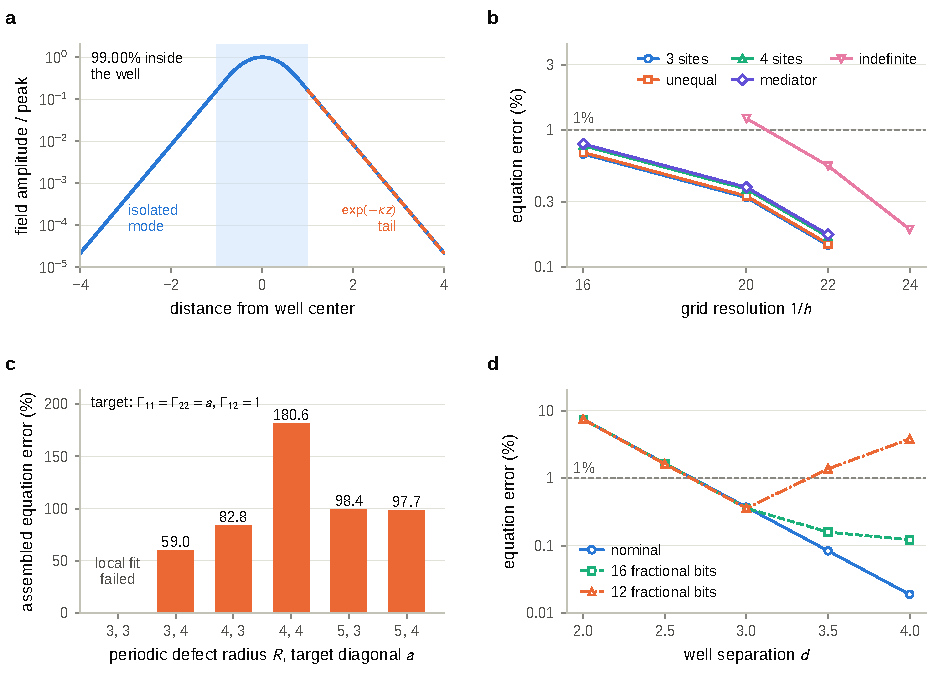
\includegraphics[width=\linewidth]{figures/si/numerical_controls.pdf}
\caption{\textbf{Confinement, assembly and material precision in the numerical examples.}
\textbf{a}, Isolated-waveguide field amplitude, normalized to its peak;
shading marks the well support. The $99.00\%$ fraction refers to the unweighted
electric-field norm squared inside that support. The dashed tail has the
background cutoff exponent $\kappa=\sqrt{\pi^2-1}$.
\textbf{b}, All-input equation errors of the five prescribed waveguide targets
under full-vector refinement, including the coarsest indefinite case above
$1\%$.
\textbf{c}, Assembled periodic-device errors after calibration against local
single- and pair-component responses. The labels give defect radius $R$ and
target diagonal $a$; the first case did not meet its local-fit criterion.
\textbf{d}, Four-site waveguide errors versus separation in the fine channel
calculation. Nominal strengths and strengths rounded to 12 or 16 fractional
binary bits use identical source functions and decoder gains. Markers denote
computed cases, with connecting lines as guides.}
\label{n:fig:controls}
\end{figure}
